
\documentclass{beamer}
\DeclareGraphicsExtensions{.pdf,.png,.jpg,.eps}
\setbeamertemplate{caption}{\raggedright\insertcaption\par}


\usepackage{graphicx}

\title{MC-Cons: RNA 2D structural assignment}
\author{Gabriel C-Parent}
%\date{project name}


\usetheme{Execushares}

\begin{document}

\maketitle
\begin{frame}
	\frametitle{outline}
	\begin{center}
		\begin{itemize}
			\item what?
			\item why?
			\item how?
			\item what's next?
			\item Q\&A
		\end{itemize}
	\end{center}
\end{frame}


\begin{frame}
	\frametitle{aknowledements first}
	\begin{figure}[!htb]
	\centering
	
\includegraphics[scale=0.25]{lab.jpg}
	%\caption{these guys are awesome! thanks for everything}
	\end{figure}
\end{frame}

\section{what?}

\subsection{graphical example}

\begin{frame}
	\frametitle{so you have structures...}
\begin{figure}[!htb]
\centering
\resizebox{0.5\textwidth}{!}{\input{all_subopts.pdf_tex}}
\caption{Given secondary structures of functionally related RNAs, which ones might explain the function?}
\end{figure} 
\end{frame}



\begin{frame}
	\frametitle{now you can have consensus!}
	\begin{figure}[!htb]
	\centering
	\resizebox{0.75\textwidth}{!}{\input{consensus_example.pdf_tex}}
	\caption{Let's suppose that their function is explained by a subset of similar structures (consensus). \\\hspace{\textwidth}In this case, 2 consensus make sense. Sometimes you get more, sometimes you get less.}
	\end{figure} 
\end{frame}



\section{why?}

\begin{frame}
	\frametitle{what's the point?}
\begin{figure}[!htb]
\centering
\resizebox{0.55\textwidth}{!}{\input{consensus_banner.pdf_tex}}
\end{figure} 

	\begin{itemize}
		
		\item goal: finding common/similar structures within suboptimal secondary structures
		\item useful for
		\begin{itemize}
			\item improving secondary structure prediction for functionally related RNAs
			\item exploring shared alternative structures
		\end{itemize}
	\end{itemize}
	
\end{frame}


\section{how?}

\subsection{general workflow}
\begin{frame}
	\frametitle{workflow}
	\begin{columns}
		\column{0.38\linewidth}
		\centering
		\begin{figure}[!htb]
			\resizebox{1.\textwidth}{!}{\input{workflow.pdf_tex}}
		\end{figure} 
        
        \column{0.58\linewidth}
        \begin{itemize}
        		\item a consensus minimizes the sum of pairs of distances between objects
        		\item optimization steps
        		\begin{enumerate}
        		        			\item base pair structural similarity (modified tree edit distance)
        			\item string edit distance on Vienna dot-bracket representation
        		\end{enumerate}
			\item two solver in C++ (branch \& bound and genetic algorithm)
        \end{itemize}
         \end{columns}
         
\end{frame} 


\subsection{matching base pairs}
\begin{frame}
	\frametitle{first match base pairs}
	\begin{figure}[!htb]
	\centering
	\resizebox{0.4\textwidth}{!}{\input{bp_tree.pdf_tex}}
	\end{figure} 
	
	\begin{itemize}
		\item base pair trees created (many-to-one function)
		\item unit tree indel distance calculates number of base pairs to add or remove to transform a tree into another
	\end{itemize}
	

\end{frame}



\subsection{match the bulges}
\begin{frame}
	\frametitle{then match unpaired}
	\begin{figure}[!htb]
	\centering
	\resizebox{0.75\textwidth}{!}{\input{tree_filtering.pdf_tex}}
	\end{figure}	
	\begin{itemize}
		\item filtered by tree structure, now refine
		\item placing the bulges around the skeleton...
		\item string edit distance on dot-bracket
	\end{itemize}
\end{frame}



\section{examples}
\subsection{IREs}
\begin{frame}
	\frametitle{IREs}
	\begin{figure}[!htb]
	\centering
	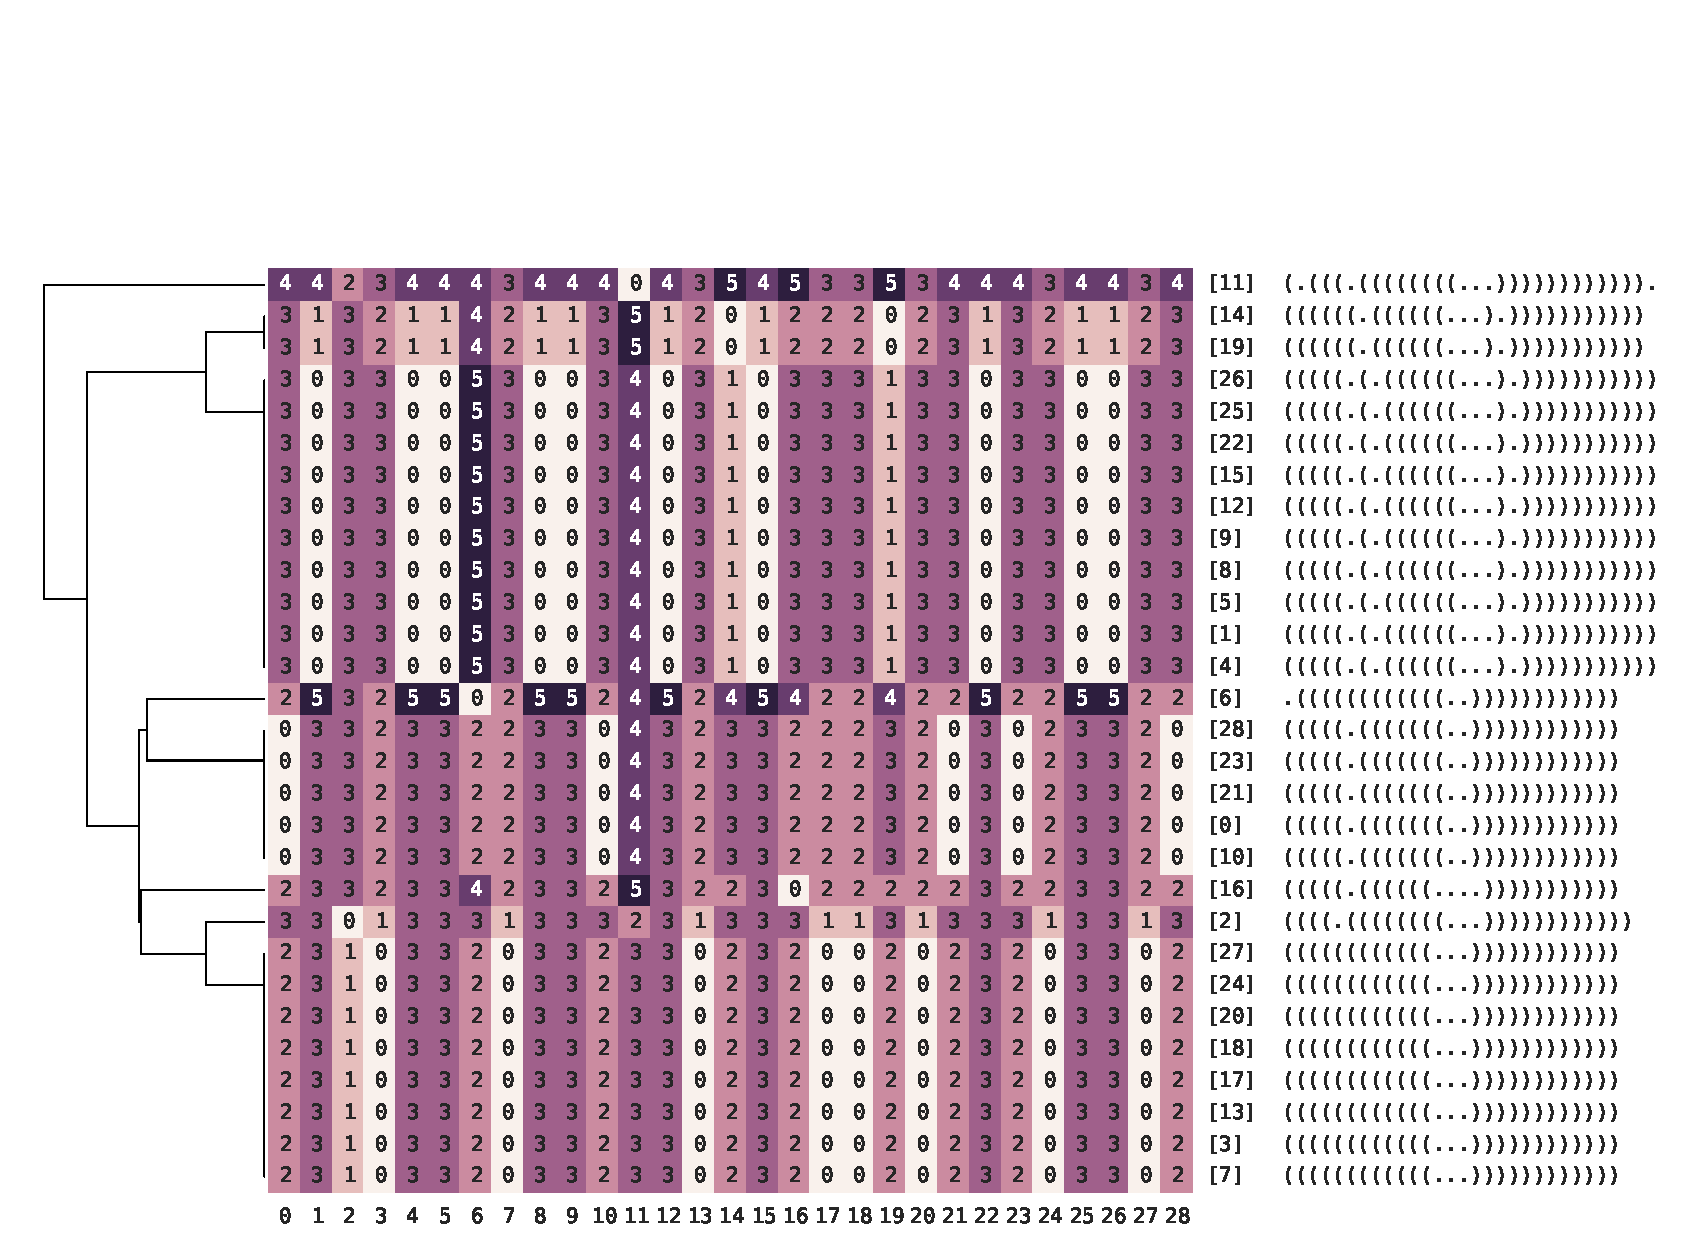
\includegraphics[scale=0.25]{figs/ires10.eps}
	\caption{IREs structural assignment given 50 suboptimal for 29 different IREs.}
	\end{figure} 
\end{frame}



\subsection{tRNAs}
\begin{frame}
	\frametitle{tRNAs}
	

\end{frame}


\section{what's next?}
\begin{frame}
	\frametitle{future work}
	\begin{itemize}
		\item MC-Cons improvements
		\begin{itemize}
			\item parallelization
			\item better distance functions?
			\item heuristic improvement?
		\end{itemize}
		
		\item derivative works
		\begin{itemize}
			\item base pair tree constraints/masks
			\item 3D to 2D tree distance
		\end{itemize}				

	\end{itemize}
\end{frame}



\section{recap}

\begin{frame}
	\frametitle{recap}
	\begin{itemize}
		\item MC-Cons creates RNA 2D structural assignment
		\item useful for finding structures explaining function
		\item available at \url{https://github.com/major-lab/MC-Cons}
	\end{itemize}
\end{frame}

\section{Q\&A}

\begin{frame}
	\frametitle{Q\&A}
		\url{https://github.com/major-lab/MC-Cons}
\end{frame}




\end{document}